\section{Interfaccia utente}
\subsection{Sezioni comuni}
Tutte le pagine dell'applicazione sono caratterizzate da un layout comune, che
include:
\begin{itemize}
    \item \textbf{Intestazione:} contiene il logo del progetto e il titolo dell'applicazione;
    \item \textbf{Contenuto principale:} è la sezione centrale della pagina, in cui viene visualizzato il contenuto specifico della pagina;
    \item \textbf{Piè di pagina:} contiene informazioni sul copyright e i link ai profili social del progetto;
\end{itemize}
\begin{figure}[ht!]
    \centering
    
\includegraphics[scale=0.6]{template/images/placeholder.png}
    \caption{Sezioni comuni}
\end{figure}

\subsection{Homepage}
La homepage è la prima schermata che l'utente visualizza all'apertura
dell'applicazione. L'elemento principale è un menu a tendina, situato al centro
della pagina: esso contiene una lista di dataset, ognuno dei quali rappresenta
un argomento di studio diverso. Scegliendo un'opzione dal menu, l'utente può
visualizzare le informazioni relative a quel dataset:
\begin{itemize}
    \item Nome del dataset;
    \item Breve descrizione del dataset;
    \item Dimensioni del dataset (numero di righe e colonne);
    \item Link all'ambiente 3D associato al dataset.
\end{itemize}
L'utente può espandere ciascun elemento della
lista per accedere a una vista dettagliata con maggiori informazioni. Una volta
selezionato un dataset, l'utente dovrà attendere il caricamento dei dati. Al
termine, verrà reindirizzato all'ambiente 3D.

\begin{figure}[ht!]
    \centering
    
\includegraphics[scale=0.6]{template/images/placeholder.png}
    \caption{Homepage}
\end{figure}

\subsection{Ambiente 3D}
L'ambiente 3D è la schermata principale in cui l'utente può visualizzare i dati
e interagire con essi. La pagina comprende i seguenti elementi:
\begin{itemize}
    \item \textbf{Grafico 3D:} rappresenta il dataset selezionato e consente di
          interagire con esso;
    \item \textbf{Form delle opzioni:} può essere reso visibile premendo
          il pulsante situato in alto a destra. Consente di filtrare i dati in
          base a criteri specifici e modificare le opzioni di visualizzazione;
    \item \textbf{Tabella dei dati:} può essere resa visibile premendo il
          pulsante in basso a sinistra. Mostra il dataset in forma tabellare e
          consente di interagire con esso.
\end{itemize}
\begin{figure}[ht!]
    \centering
    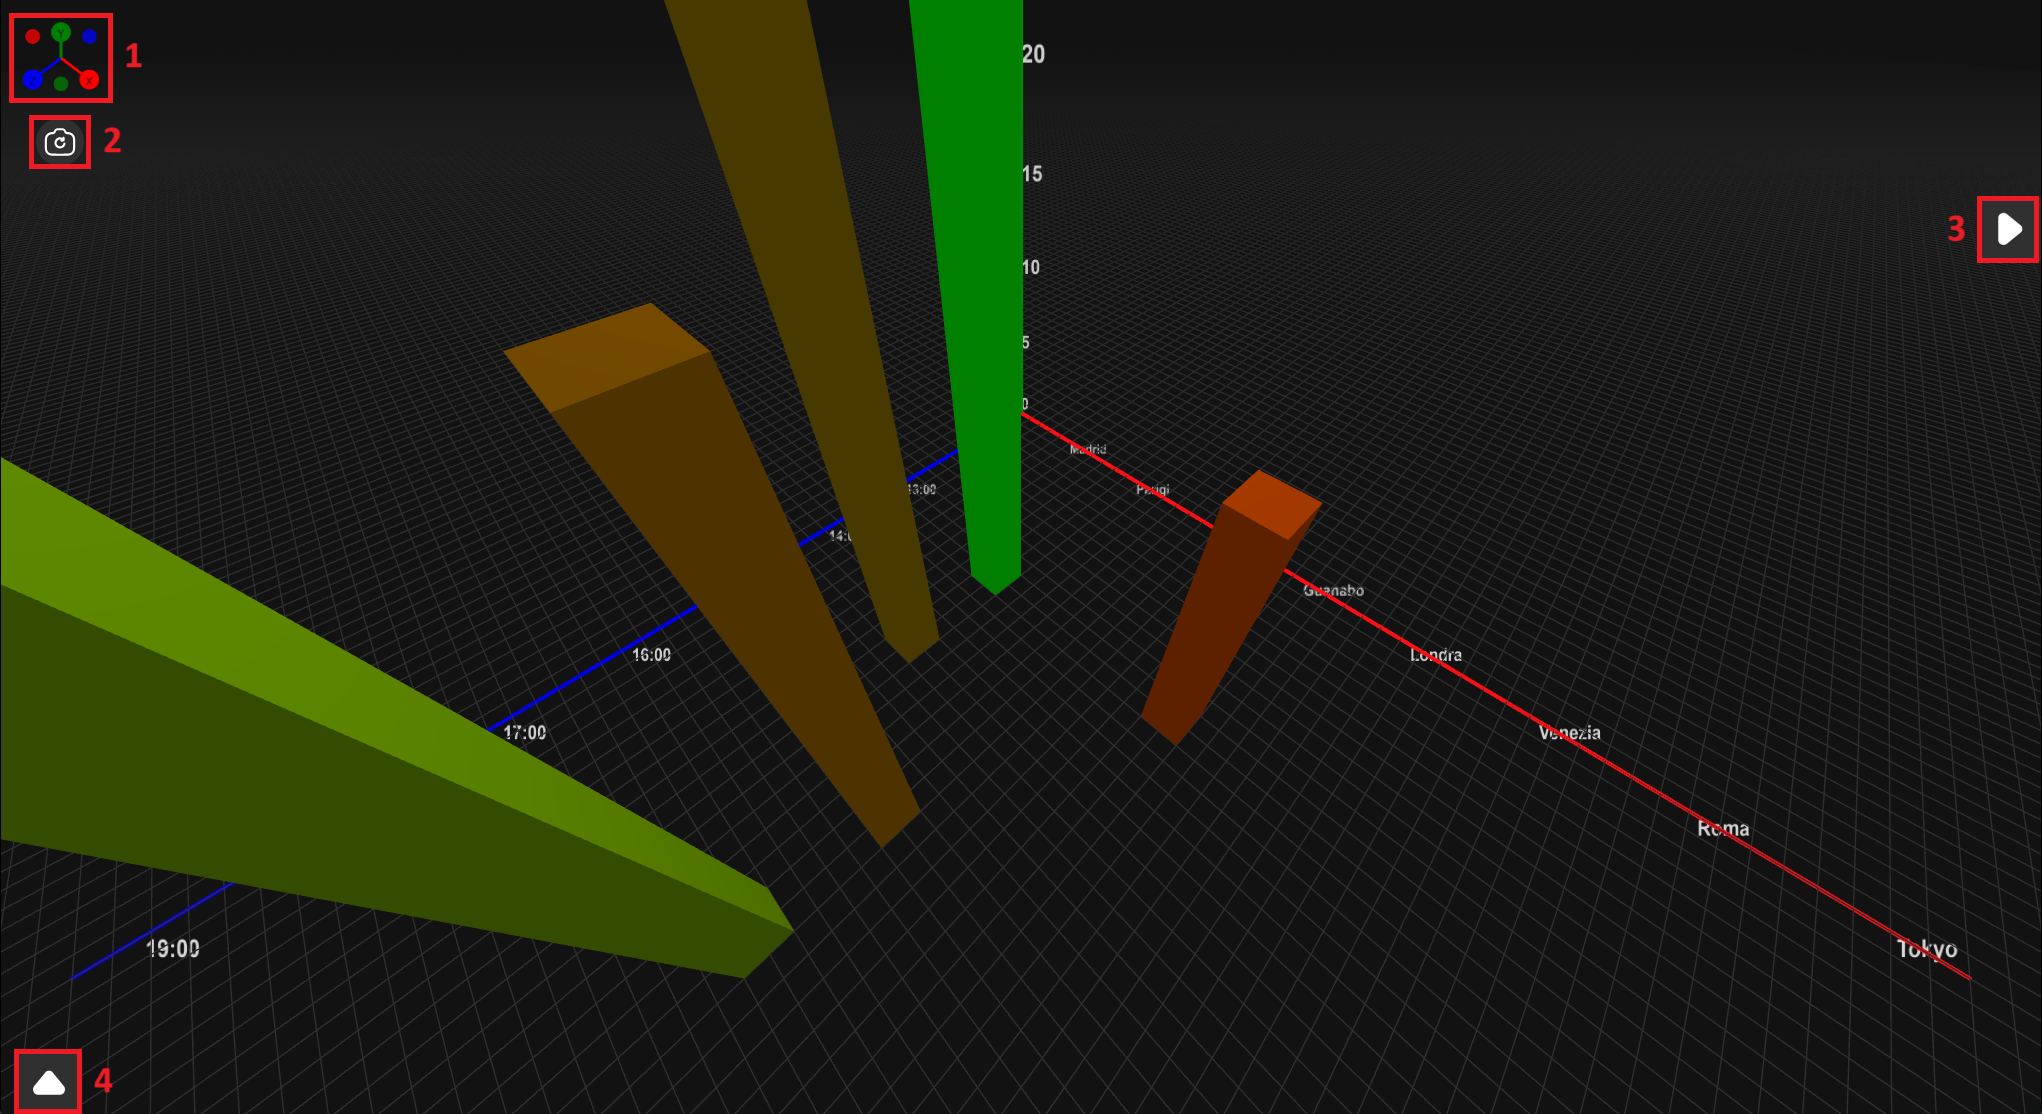
\includegraphics[scale=0.29]{template/images/envpage.png}
    \caption{
        Ambiente 3D con elementi interattivi numerati:\\
        (1) Gizmo;\\
        (2) Pulsante di reset della visualizzazione;\\
        (3) Pulsante per il form delle opzioni;\\
        (4) Pulsante per la tabella.
    }
\end{figure}
\subsubsection{Grafico 3D}
Il grafico 3D è l'elemento centrale dell'ambiente 3D e rappresenta il dataset
selezionato. Ogni barra del grafico rappresenta un valore specifico del
dataset, mentre l'altezza della barra indica il valore stesso. Le barre sono
colorate in base al loro valore, con una scala di colori che va dal rosso
(valori bassi) al verde (valori alti).

\paragraph{Navigazione 3D}
All’interno dell'ambiente 3D l'utente può interagire con il grafico con le
seguenti modalità:
\begin{itemize}
    \item \textbf{Spostamento:} l'utente può spostare il grafico senza cambiarne
          l'angolazione tenendo premuto il tasto destro del mouse e trascinando
          nella direzione desiderata;
    \item \textbf{Zoom:} l'utente può ingrandire o ridurre il grafico
          utilizzando la rotellina del mouse o il gesto di pinch sul touchpad;
    \item \textbf{Rotazione:} l'utente può ruotare il grafico senza spostarlo
          tenendo premuto il tasto sinistro del mouse e trascinando nella direzione desiderata;
\end{itemize}
Questi controlli sono sempre attivi quando il cursore è sopra il grafico.
\begin{figure}[ht!]
    \centering
    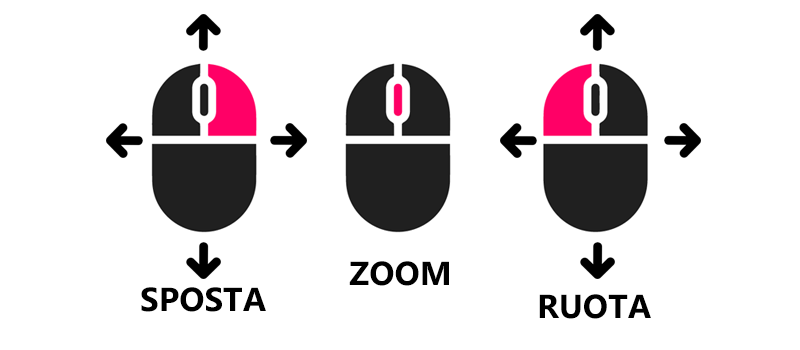
\includegraphics[scale=0.6]{template/images/comandi.png}
    \caption{Comandi per la navigazione}
\end{figure}

\paragraph{Navigazione avanzata}
L'utente può usufruire di funzionalità avanzate per la navigazione del grafico
3D:
\begin{itemize}
    \item \textbf{Rotazione tramite gizmo:} l'utente può ruotare il grafico
          senza spostarlo tenendo premuto il tasto sinistro del mouse su un'estremità
          dell'asse nel gizmo e trascinando nella direzione desiderata;
    \item \textbf{Reset:} l'utente può riportare il grafico alla posizione
          iniziale premendo il pulsante di reset della
          visualizzazione in alto a sinistra, sotto al gizmo.
\end{itemize}
\begin{figure}[ht!]
    \centering
    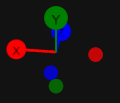
\includegraphics[scale=0.6]{template/images/gizmo.png}
    \hspace{1cm}
    
\includegraphics[scale=0.6]{template/images/resetcam.png}
    \caption{Elementi per la navigazione avanzata}
\end{figure}

\subsubsection{Form delle opzioni}
Il form delle opzioni consente di filtrare i dati in base a criteri specifici e
modificare le opzioni di visualizzazione. Può essere reso visibile oppure
nascosto premendo il pulsante situato in alto a destra dell'ambiente 3D.
Procedendo dall'alto verso il basso, il form è composto da:
\begin{itemize}
    \item Pulsante per filtrare i valori superiori o inferiori (a seconda dell'opzione
          selezionata) al valore medio del dataset;
    \item Campo di input per inserire un numero intero positivo;
    \item Pulsante per filtrare i primi N valori più alti o più bassi (a seconda
          dell'opzione selezionata) del dataset, dove N è il numero inserito nel campo di
          input;
    \item Pulsanti di opzione per scegliere se filtrare i valori più alti o più bassi,
          relativamente a qualunque filtraggio;
    \item Pulsante per rimuovere il filtro applicato;
    \item Pulsanti di opzione per scegliere se visualizzare o meno il piano parallelo al
          piano XZ (base del grafico), che mostra il valore medio del dataset.
\end{itemize}
\begin{figure}[ht!]
    \centering
    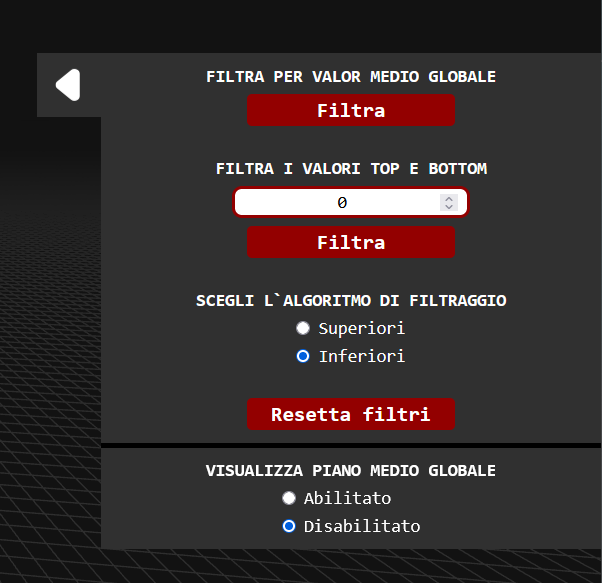
\includegraphics[scale=0.6]{template/images/options.png}
    \caption{Form delle opzioni}
\end{figure}

\subsubsection{Tabella dei dati}
La tabella dei dati mostra il dataset in forma tabellare e consente di
interagire con esso. Può essere resa visibile oppure nascosta premendo il
pulsante situato in basso a sinistra dell'ambiente 3D.\\ La prima colonna della
tabella contiene le intestazioni delle righe, che rappresentano le etichette
dell'asse X del grafico. La prima riga della tabella contiene le intestazioni
delle colonne, che rappresentano le etichette dell'asse Z del grafico. Le celle
della tabella contengono i valori del dataset e possono assumere colori diversi
a seconda che la corrispondente barra del grafico sia visibile o meno.\\
L'utente può premere su una cella per filtrare i valori superiori o inferiori
(a seconda dell'opzione selezionata) al valore della cella stessa.
\begin{figure}[ht!]
    \centering
    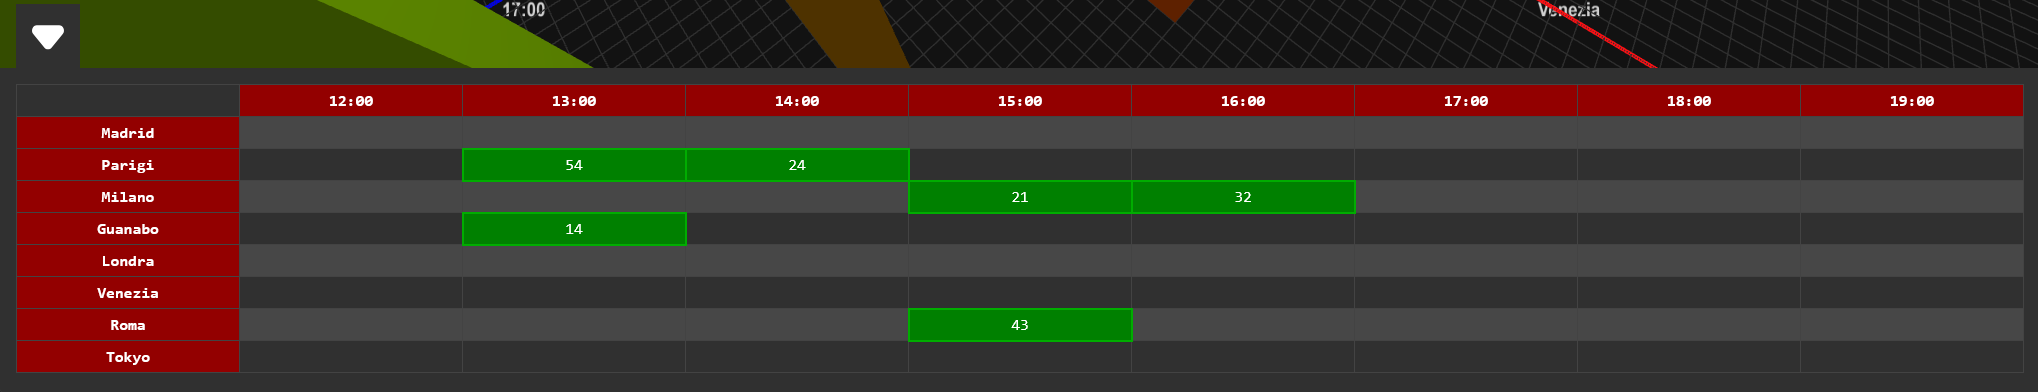
\includegraphics[scale=0.29]{template/images/table.png}
    \caption{Tabella dei dati}
\end{figure}